2012年,Alexnet\cite{krizhevsky2012imagenet}によって畳み込みニューラルネットワークを用いた画像認識手法がこれまでの既存の手法を遥かに上回る性能を提示して以来,コンピュータビジョンの分野において畳み込みニューラルネットワーク(Convolutional Neural Netowrk : CNN)を用いたアルゴリズムは必要不可欠な手法となった.
畳み込みニューラルネットワークとは,コンピュータビジョンの分野において,現在最も成果を挙げているニューラルネットワークの構造の一つである.
畳み込みニューラルネットワークは畳み込み層とプーリングと呼ばれる演算を中心に構成されるネットワークである.
本節では,畳込みニューラルネットワークの基礎から,著名なモデルの解説まで行う.

\subsection{畳み込み演算}
    本項では,畳み込みニューラルネットワークにおける畳み込み演算について説明する.
    畳み込みニューラルネットワークにおける畳み込み演算は,以前からコンピュータビジョンの分野において画像から特徴量を抽出するために使われている手法をベースとしている.
    畳み込み演算は,画像処理におけるフィルター演算に相当する.
    このフィルターという言葉は,カーネルと表現されることもある.
    畳み込みニューラルネットワークはある特定のテクスチャパターンに反応するように学習されたフィルタを,入力データに対して畳み込み演算をすることで特徴の抽出を行う.
    \begin{figure}[ht]
      \centering
      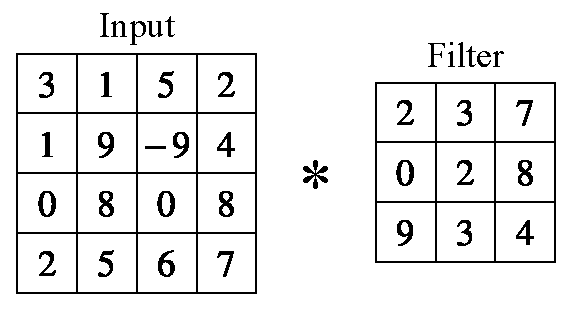
\includegraphics[width=10cm]{8_appendix/img/conv.pdf}
      \caption{Ex) input and filter for convolution.}
      \label{fig:ex_conv_input_filter}
    \end{figure}
    
    ここで例として,入力データが$4 \times 4$の2階のテンソルであり,フィルタのサイズが$3 \times 3$の2階のテンソルである場合を考える.
    このときの畳み込み演算の概要図を\ref{fig:ex_conv_input_filter}に示した.
    また畳み込み演算の計算の過程の模式図を\ref{fig:ex_conv_step_1}から\ref{fig:ex_conv_step_4}に示した.
    入力データからフィルタと同サイズのテンソルを抽出し,それらとフィルタの要素ごとの積(アダマール積$\odot$)を計算した後,その和を計算結果とする.
    これを位置を$N$ピクセルずつずらしながら繰り返し,その位置ごとの結果をまとめたテンソルが出力となる.
    ここで,ずらす量のことストライドと呼ぶ.
    
    \begin{figure}[ht]
      \centering
      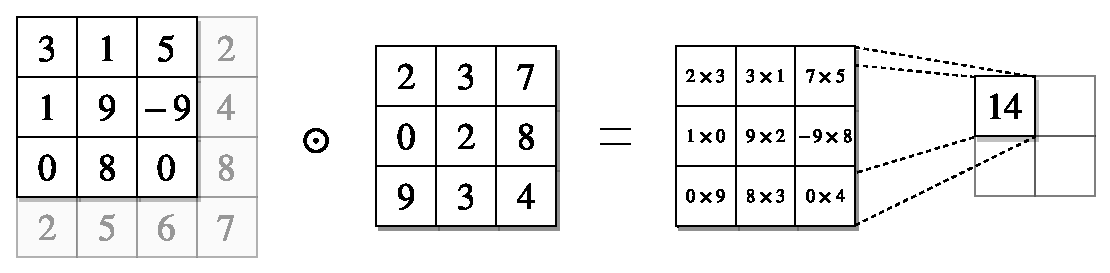
\includegraphics[width=14cm]{8_appendix/img/conv_step_1.pdf}
      \caption{Outline of convolution (Step-1).}
      \label{fig:ex_conv_step_1}
    \end{figure}
    \begin{figure}[ht]
      \centering
      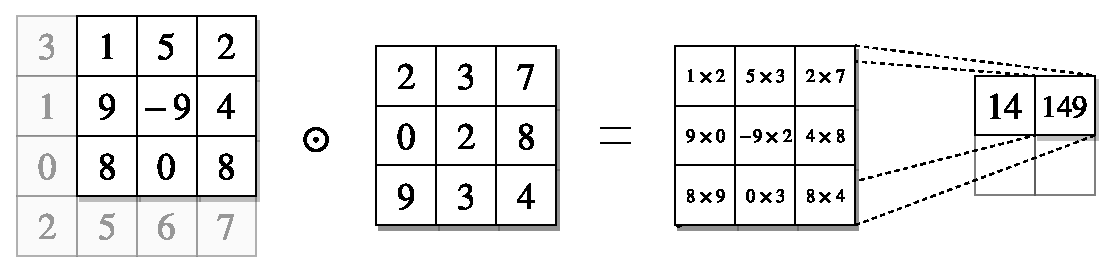
\includegraphics[width=14cm]{8_appendix/img/conv_step_2.pdf}
      \caption{Outline of convolution (Step-2).}
      \label{fig:ex_conv_step_2}
    \end{figure}
    \begin{figure}[ht]
      \centering
      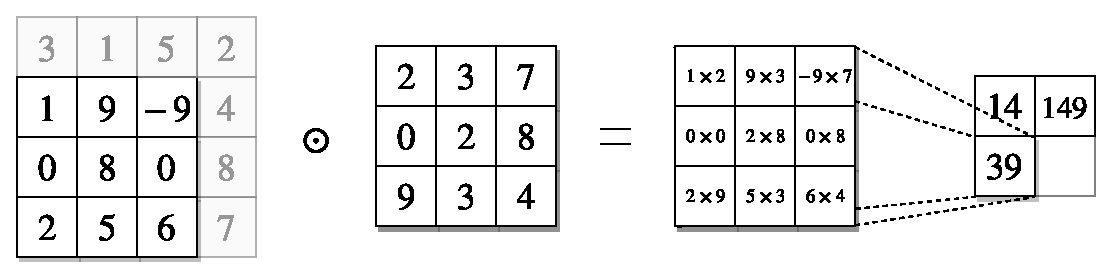
\includegraphics[width=14cm]{8_appendix/img/conv_step_3.pdf}
      \caption{Outline of convolution (Step-3).}
      \label{fig:ex_conv_step_3}
    \end{figure}
    \begin{figure}[ht]
      \centering
      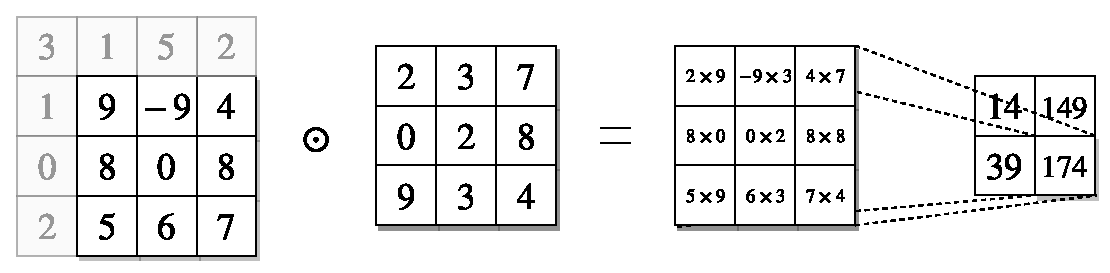
\includegraphics[width=14cm]{8_appendix/img/conv_step_4.pdf}
      \caption{Outline of convolution (Step-4).}
      \label{fig:ex_conv_step_4}
    \end{figure}
    ニューラルネットワークの学習においては,この畳み込みを行うフィルタの各要素のパラメータが学習される.
    一方で,フィルタの形状,大きさやフィルタの位置をずらす量等のパラメータは学習したいデータや抽出したい特徴から設計する必要がある.
    また一般的な畳み込みニューラルネットワークでは,図\ref{fig:outline_of_convolution_3d}のように入力データに対して複数のフィルタを用いて畳み込み演算を行うため,その出力結果は3階のテンソルとなる.
    さらに,畳込み演算の結果に対して更に畳み込み演算が適用されることが多い.例えば,2次元画像を入力データとした場合,そのデータ形状はチャンネル $\times$ 高さ $\times$ 幅となる.
    \begin{figure}[ht]
      \centering
      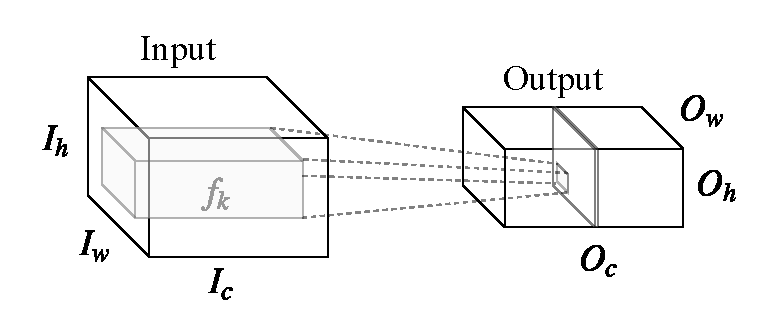
\includegraphics[width=14cm]{8_appendix/img/outline_of_convolution_3d.pdf}
      \caption{Outline of convolution.(3D)}
      \label{fig:outline_of_convolution_3d}
    \end{figure}

    ここで,1つのフィルタで畳込み演算された結果は各チャンネルで加算されることに注意したい.
    また,畳込み演算において,バイアスはフィルタ内の共通のパラメータとして扱われることが多く,演算結果の全ての値に対して適用されることが多い.
    
    重要な点として,畳み込みニューラルネットワークは,多層パーセプトロンと比べてパラメータ数が非常に少ないことが挙げられる.
    多層パーセプトロンでは一つのユニットが次の層のすべてのユニットに結合される全結合層(fully-connected layer)のみを用いて構成されている.
    それ故に, 深い構造になるほどパラメータ数が膨大になり, 学習が困難になる.
    例えば,256$\times$256サイズの画像を入力し,次の層が100ユニットの全結合層だった場合,必要なパラメータは256$\times$256$\times$100となり,膨大な数のパラメータが必要になる.
    一方,カーネルサイズが3,チャンネル数が100の畳み込み演算を行う場合,必要なパラメータは3$\times$3$\times$100と,非常に少ないパラメータでモデルを構成することができる.
    
    \begin{figure}[ht]
        \begin{center}
            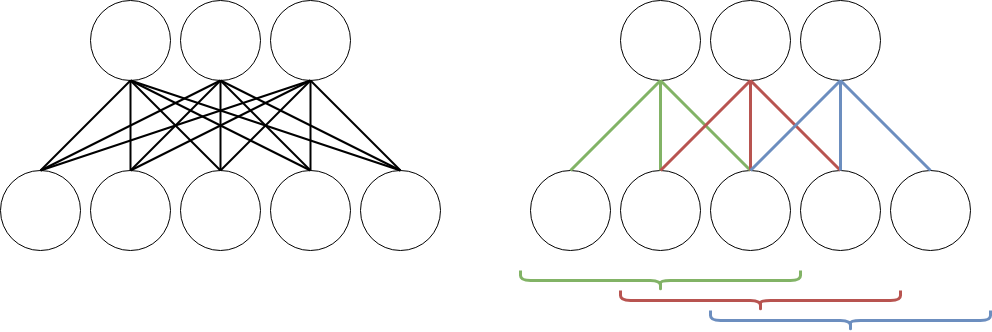
\includegraphics[width=12.0cm]{./8_appendix/img/FCL_conv.png}
            \caption{Comparison of the number of parameters in fully connected layer and convolutional layer.}
            \label{FCL_conv}
        \end{center}
    \end{figure}
    
    また,図\ref{FCL_conv}からも分かる通り, 単純な畳込み操作では画像の最も端にある画素が無くなってしまう.
    この量はカーネルサイズを$k$とすると$k-1$であり,両端で$(k-1)/2$画素の欠損が起こる.
    そのため, 画像サイズを保つためには予め同じだけの画素を付与する必要があり, その操作をパディングと呼ぶ.
    通常は0でパディングを行い,これを特にゼロパディングと呼ぶ.
    ゼロパディングでは, 画像の端の特徴マップが暗くなるなどの欠点もある.

    \begin{figure}[ht]
        \begin{center}
            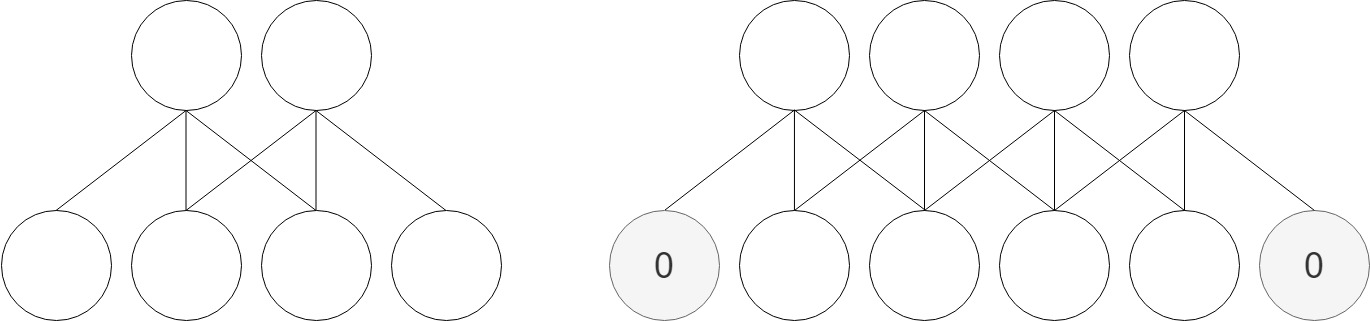
\includegraphics[width=12.0cm]{./8_appendix/img/padding.jpg}
            \caption{Image size can be maintained by zero padding.}
            \label{padding}
        \end{center}
    \end{figure}
    
    また,畳み込み層では実用上カーネルサイズは3が採用されることが多い.
    これは,カーネルサイズが3以上の畳み込み層は,カーネルサイズ3の畳み込みそうを複数重ねることにより表現可能なことに起因する.
    例えば,カーネルサイズが5の畳み込み層はカーネルサイズ3の畳込み層2つを直列に接続した場合と受容野の広さが同一である.

    ここでさらに,畳込み層のパラメータ数に着目する.
    以下に,通常の畳み込み層が持つパラメータ数を示す.
    \begin{equation}
        N_p=c_i\cdot k^2\cdot c_o
    \end{equation}
    ここで,$c_i,c_o$は入出力時のチャンネル数を表す.

    カーネルサイズ3の畳み込み層2つのパラメータ数が$2\times3^2c_i c_o$で表されるのに対して,カーネルサイズ5の畳み込み層のパラメータ数は$5^2c_i c_o$と,$(2\times 3^2)/5^2$ほど小さくなる.
    以上より,カーネルサイズが小さい畳込みを複数続けた場合,パラメータ数が少なくなる上,カーネルサイズが大きい場合と同様の効果が期待できる.
    上記の理由から,近年ではほとんどのモデルにおいて,畳み込み層のカーネルサイズは3に設定されていることが分かる.
    
\subsection{様々な畳み込み演算}
    前項では畳み込み演算の仕組みについて触れたが,近年では様々な畳込み手法が提案されている.
    ここでは,特殊な畳み込みとして,特に本論文で用いる畳み込みの5つを示す.
    
    \subsubsection{Dilated Convolution}
    Dilated Convolutionは広げられた(dilated)範囲を畳み込む方法で,通常の畳み込みよりも大域的特徴を一度に捉えることができる.
    この手法は一部でAtrous畳み込みとも呼ばれている.
    Dilated filterのアイデアは効率的なウェーブレット分解のためのアルゴリズム\cite{holschneider1990real}としてで開発され,画像のセグメンテーションなどの予測などで利用されている\cite{huang2017densely,lin2014microsoft}.
    通常の畳み込みは,大域的な特徴を捉えるためにカーネルサイズ$k$を大きくすると,$k$の二乗に比例してパラメータ数が増加する.
    そこで,以下のように入力するピクセルの間隔を空けることにより,通常の畳み込みと同様のパラメータで,より大域的な情報を畳み込むことが可能となった.
    \begin{figure}[ht]
        \begin{center}
            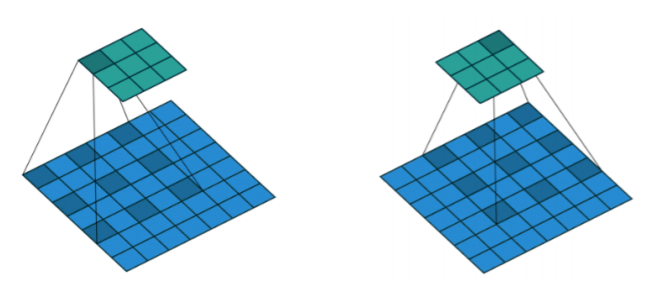
\includegraphics[width=12.0cm]{./8_appendix/img/dilated_conv}
            \caption{Dilated Convolution.}
        \end{center}
    \end{figure}

    \subsubsection{Transposed Convolution}
    Transposed Convolution(転置畳み込み)は,アップサンプリングする際に用いられる手法であり,Deconvolution(逆畳み込み)とも呼ばれる.
    他の畳込み演算と異なり、出力される画像サイズが元の画像よりも大きくなる.
    \begin{figure}[ht]
        \begin{center}
            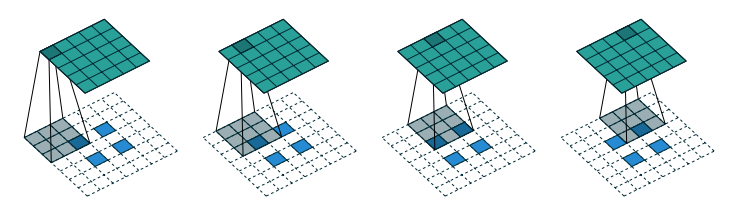
\includegraphics[width=15.0cm]{./8_appendix/img/Deconvolution}
            \caption{Transposed Convolution.}
        \end{center}
    \end{figure}

    \subsubsection{Depthwise Convolution}
    Depthwise ConvolutionはMobileNet\cite{howard2017mobilenets}において採用されている,CNNのパラメータ削減のために導入されている畳み込みの1つである.
    
    通常,畳み込み層では畳込み演算を行った後に各演算結果をチャンネル方向に加算する.
    つまり,入力された全部のチャンネルに対し,単一のフィルタが計算を行っている.
    一方,Depthwise Convolutionでは各チャンネルごとにに対応するフィルタが決まっており,これにより計算量が$1/c_i$となる.
    これはチャンネル間の相関を無視して,単純に空間的な畳込みを実行していることになる.
    
    \subsubsection{Pointwise Convolution}
    Pointwise ConvolutionはDepthwise Convolutionと同様に,MobileNet\cite{howard2017mobilenets}において採用されているCNNのパラメータ削減のために導入されている畳み込みの1つである.
    
    通常の畳み込みではカーネルサイズ$k$を大きくすると,$k$の二乗に比例してパラメータ数が増加する.
    つまり,この$k$を$k=1$と固定することにより,パラメータ数を$1/k^2$とすることができる.
    この畳込みは$k=1$であるため,空間的特徴を捉えずに,チャンネル間の相関構造だけを変化させる特殊な畳み込み演算である.
    また,この畳込みの重要な点として,チャンネル数を変化させることが可能であるため,チャンネル数の辻褄を合わせるような際に良く利用される.
    
    \subsubsection{Depthwise Separable Convolution}
    Depthwise Separable Convolution,MobileNet\cite{howard2017mobilenets}において主に採用されている畳み込み手法である.
    この手法は前述したDepthwise ConvolutionおよびPointwise Convolutionを直列に接続した畳み込みのことを指す.

    Depthwise Convolutionは非常に軽量だが,チャンネル間の構造を捉えることができない上に,出力のチャンネル数が$c_o=c_i$と固定されてしまう.
    そのため,Pointwise Convolutionと縦続接続することでチャンネル側の相関を取り,後に扱いやすいようにチャンネル数の調整を行う.

    パラメータ数はDepthwise ConvolutionおよびPointwise Convolutionの加算となるため,以下のようになる.
    \begin{equation}
        N_p = c_i k^2 + c_i c_o = c_i (k^2 + c_o)
    \end{equation}
    以上により,通常の畳み込みと比べて,Depthwise Separable Convolutionを利用することによるパラメータの削減率は以下の通りである.
    \begin{equation}
        \frac{k^2 + c_o}{k^2 c_o}
    \end{equation}
    これは,ほとんどの層で$c_o>64$かつ$k=3$と設定されていることを踏まえると,全体のパラメータ数がおよそ$1/9$に削減されることを表している.

\subsection{プーリング演算}
    プーリング演算とは,層が深くなるにつれて増大する学習パラメータを削減し,更に畳み込み演算によって得られ特徴量から重要な特徴量を取り出す等の処理を行う演算である.
    この演算を行う層をプーリング層という.
    ここでは,畳み込みニューラルネットワークにおいて最も使われるプーリング演算の例として,マックスプーリング(max pooling)について説明する.
    前述した$4 \times 4$の2階のテンソルに対してマックスプーリング演算を行う.
    このときの演算の概要図を\ref{fig:ex_maxpooling_step_1}-\ref{fig:ex_maxpooling_step_4}に示した.
    \begin{figure}[ht]
      \centering
      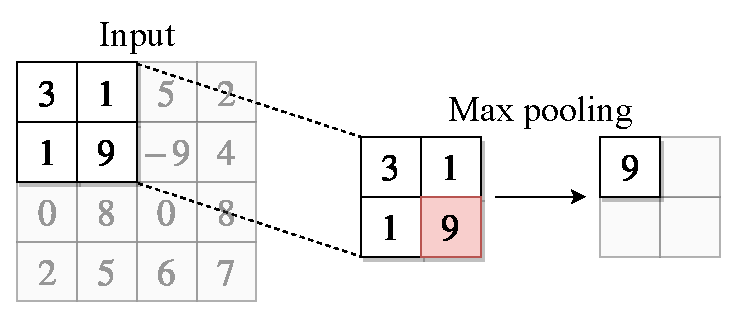
\includegraphics[width=8cm]{8_appendix/img/max_pooling_step1.pdf}
      \caption{Outline of max pooling (Step-1).}
      \label{fig:ex_maxpooling_step_1}
    \end{figure}
    \begin{figure}[ht]
      \centering
      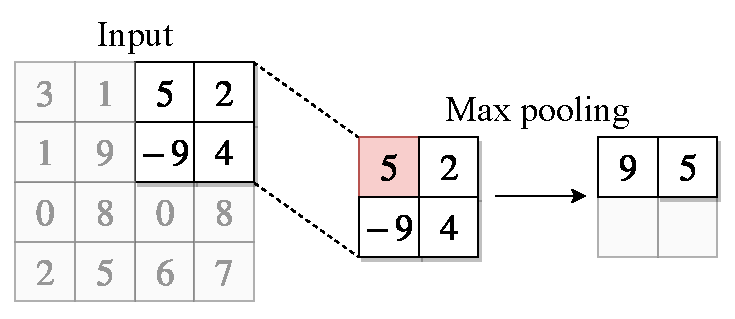
\includegraphics[width=8cm]{8_appendix/img/max_pooling_step2.pdf}
      \caption{Outline of max pooling (Step-2).}
      \label{fig:ex_maxpooling_step_2}
    \end{figure}
    \begin{figure}[ht]
      \centering
      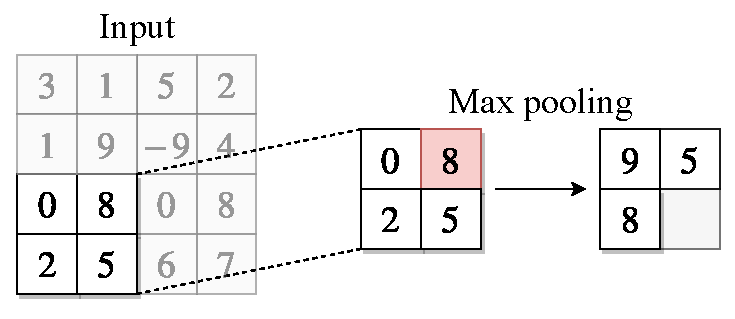
\includegraphics[width=8cm]{8_appendix/img/max_pooling_step3.pdf}
      \caption{Outline of max pooling (Step-3).}
      \label{fig:ex_maxpooling_step_3}
    \end{figure}
    \begin{figure}[ht]
      \centering
      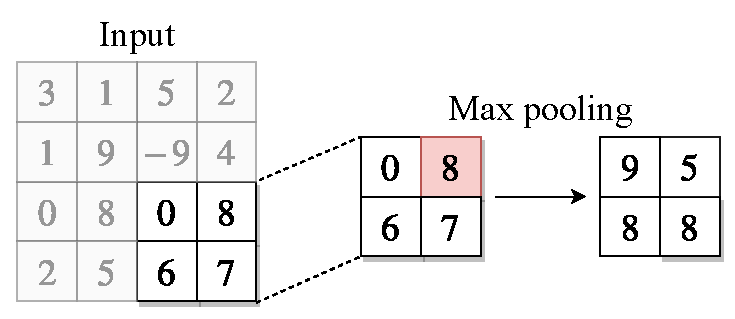
\includegraphics[width=8cm]{8_appendix/img/max_pooling_step4.pdf}
      \caption{Outline of max pooling (Step-4).}
      \label{fig:ex_maxpooling_step_4}
    \end{figure}
    図から明らかなように,入力テンソルから$2 \times 2$の大きさのテンソルを抽出し,その中で最も大きな値を出力する演算である.
    マックスプーリングでの出力は,これを位置をずらしながら繰り返し,その位置ごとにまとめたテンソルとなる.
    また, プーリング層と畳込み層の最も重要な違いは更新されるパラメータを含んでいない点である.
    マックスプーリングはカーネル中の最大値を出力したが,他によく用いられるアベレージプーリングでは,カーネル中の平均値を出力するような設計になっている.

\subsection{様々なプーリング演算}
    前項ではプーリング演算の仕組みについて触れたが,畳み込み層と同じく,近年では様々なプーリング手法が提案されている.
    ここでは,特殊なプーリング演算として,特に本論文で用いる2つのプーリング演算を示す.
    
    \subsubsection{Global Average Pooling}
    Global Average Pooling (GAP)は,入力された特徴マップについて,チャンネルごとに平均を取るプーリング演算である.
    よって,特徴マップは幅および高さを失い,ただのベクトルとして出力される.
    近年は,出力層の手前に配置されるだけではなく,アテンション機構の一部として利用された例などがある\cite{hu2018squeeze}.
    
    \subsubsection{空間ピラミッドプーリング}
    空間ピラミッドプーリング\cite{he2015spatial}(SPP, spatial pyramid pooling)は,入力画像サイズが異なっている場合でも,出力のサイズが同じになるようなプーリング層である.
    このプーリング層では,画像を格子状($1\times1, 2\times2, 4\times4, 16\times16$, ...)に分割し,それぞれでマックスプーリングを行う.
    その後,それぞれの出力値を結合し,結合したベクトルがSPPの出力となる.
    出力サイズはピラミッドのサイズ及びチャンネル数で定義される.
    \begin{figure}[ht]
        \begin{center}
            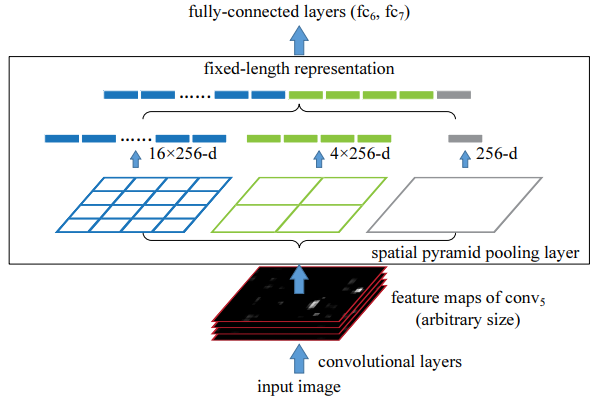
\includegraphics[width=12.0cm]{./8_appendix/img/SPP}
            \caption{spatial pyramid pooling\cite{he2015spatial}.}
        \end{center}
    \end{figure}
    

    